\BigLetter{A}{ progressively} increasing challenge in high performance and scientific computing (HPC) is how to store the enormous amount of data on disk, efficiently, especially with the ubiquitous enthusiasm for Big Data Analysis (BDA) frameworks, within the sphere of influence. A commonly used distributed computation framework for BDA and transformation is Apache's Hadoop\cite{PageHadoop}, where data access is based on HDFS (Hadoop Distributed File System) \cite{Shvachko:2010:HDF:1913798.1914427} and the primary execution model based on MapReduce\cite{Dean:2008:MSD:1327452.1327492}. Frameworks as aforementioned are developed under other circumstances, and with another purpose, than what they are used for now, such as HPC. 
\newline

HDFS, as well as the Google File System \cite{Ghemawat:2003:GFS:945445.945450}, follows a centralized architectural master/slave organization (described in \eg \cite{Tanenbaum:2006:DSP:1202502} and briefly in \cite{Wilkinson:1998:PPT:289352}) where what is denoted as NameNode acts as the master. This server maintains attributes such as permissions and namespace tree for slaves. Also, it implements a proxy to handle operations realised on the file system at the slaves. 
\newline

Writing to the Hadoop file system can likely cause, what's known as the data residual problem (see Figure \ref{fig:data-residual}). Thus, semantically correlated or coherent data can be distributed across different servers, due to the physical distribution. Latter is implemented using a conventional file system approach, \ie fixed sized blocks of 64MB. 
\newpage

\begin{figure}
	\centering
	\hspace*{15mm}
	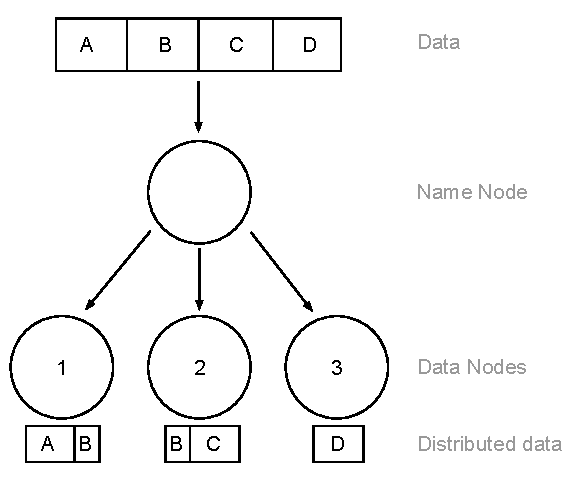
\includegraphics[scale=0.8]{pdf/data-residual.pdf}
	\caption[HDFS data residual problem]{HDFS data residual problem which ultimately requires Data Node 1 and 2 to exchange data for a consistent processing of block B, leading to an increased I/O cost. \label{fig:data-residual}}
\end{figure}

As a matter of fact, the only case where data partitioning is ensured to be avoided is when the size of the data modulo the block size is zero. As a consequence of the heretofore mentioned, individual computer scientist are necessitated to implement a network communication protocol between the slaves to handle this problem, which typically are causing increased latency. The reason is to ensure a consistent view and process of the coherent data representations.

\section{Problem definition} \label{sec:problem}
\begin{quotation}
\hspace*{-7mm}
\textit{First and foremost, analyze and investigate whether a distributed parallel file system that efficiently hides latency and reduce IO-cost is durable. Secondly, if achievable implement a prototype in a sensibly selected language, architecture and environment.} \newline
\end{quotation}

\section{Related work} \label{sec:related}
Existing implementations and research projects within the field of big data analysis frameworks and distributed parallel file systems relevant to this project will be described in this section, including the once previously mentioned.

\subsection*{Hadoop}
Hadoop was originally described in 2010 by Shvachko \etal in \cite{Shvachko:2010:HDF:1913798.1914427}. The Apache and Yahoo! developed framework is designed to store and analyze enormous datasets. It provides the distributed hierarchical file system with directories and archives HDFS (Hadoop Distributed File System), as data access layer (DAL) and a primary execution model based on the programming paradigm MapReduce (sharing this feature with the following computing platform), outlined in definition \ref{def:mapreduce}.
\vspace*{5mm}

\begin{definition}[MapReduce] \label{def:mapreduce}
\textit{A programming paradigm and an associated implementation presented by Dean and Ghemawat in} \cite{Dean:2008:MSD:1327452.1327492} \textit{used for data generation, analysis and processing. Fundamentally it is assembled by two separate user specified functions:} \texttt{map} \textit{and} \texttt{reduce}\textit{, which at execution time are parallelized automatically.}
\end{definition}

HDFS implements a master/slave architecture where the previously momentarily described NameNode server is the master, and the DataNodes are the slaves. Metadata and application data is stored separately on respectively master and slave, just as in the Google File System, examined later in this section. Having a stateful master without replication is a single point of failure  as described by Yahoo! in the Hadoop developer tutorial:

\begin{quotation}
	\textit{"The single point of failure in a Hadoop cluster is the NameNode $\ldots$ loss results in cluster unavailability. The permanent loss of NameNode data would render the cluster's HDFS inoperable."}\cite{YahooDocumentation}
\end{quotation}

Additionally it's a potential bottleneck in a system, but in this project it's a tradeoff for throughput and accessibility.

\subsection*{Facebook (Hadoop)}
The loss of a NameNode is not tolerated, as described, nor at Facebook. It is because more or less the whole Hadoop cluster is not correctly functioning if it is unavailable. Figure \ref{fig:fb-hadoop-incidents} illustrates the percentage of Hadoop related incidents at Facebooks Data Warehouse in relation to any other components. Thus improving HDFS and the single point of failure (SPOF) error at the NameNode is an essential task to ensure that the ecosystem are efficient and reliable.

\begin{figure}[h!]
	\centering
	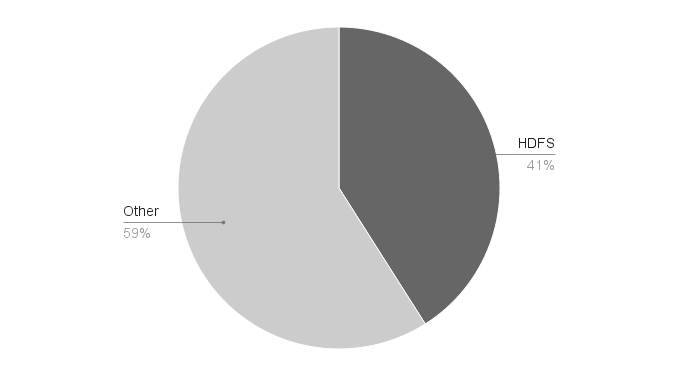
\includegraphics[scale=0.48]{img/fb-hadoop-incidents.png}
	\caption[Incidents at Facebooks Data Warehouse]{Incidents at Facebooks Data Warehouse by percentage at the responsible part, others including user specified jobs etc. \newline \textit{Statistics are from }\cite{FacebookHadoopImprovement}. \label{fig:fb-hadoop-incidents}}
\end{figure}

\newpage
Facebooks engineers designed a solution based on a so-called Avatarnode, as a functioning hot fail-over solution, turning the existing NameNode into a highly-available server. The open source Avatarnode is essentially two NameNodes wrapped in an Apache ZooKeeper\footnote{Apache ZooKeeper\cite{PageZookeper} is a centralized service provider for configuration information and naming etc.} instance, with support for manual failover. The two NameNode instances behave as an active one and a standby with internal virtual IP address (VIP), handled by ZooKeeper, \ie each client request is initialized through that to get the VIP of the primary node (see Figure \ref{fig:facebook-avatarnode}).
\newline

Synchronization between the active and the standby NameNode instance is managed by a NFS (Network File Server).
\vspace*{3mm}

\begin{figure}[h!]
	\centering
	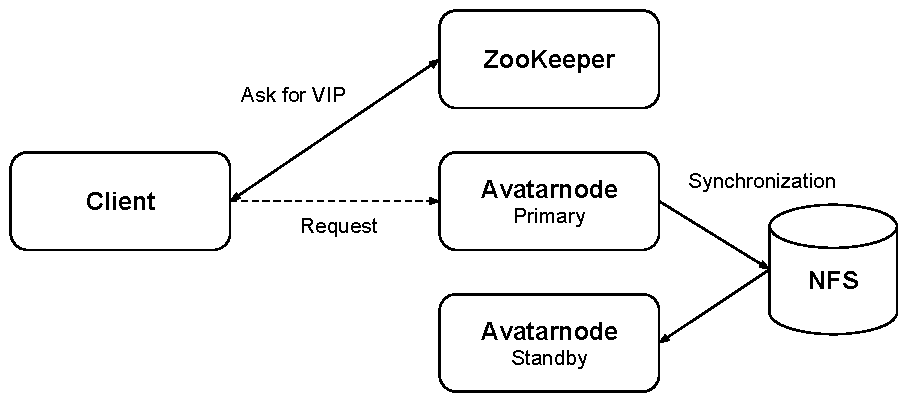
\includegraphics[scale=0.8]{pdf/facebook-avatarnode.pdf}
	\caption[Avatarnode: Facebooks Hadoop implementation]{Control flow of the AvatarNode and ZooKeeper with virtual IP address and network file server for synchronization. \label{fig:facebook-avatarnode}}
	\vspace*{3mm}
\end{figure}

Facebook claims that the solution leads to a projected result of 50\% lesser planned downtime, \ie a critical time where that part of the warehouse is unavailable. Though, one could certainly come up with new issues arising in this solution:
\begin{itemize}
	\item SPOF error reliability of the Apache ZooKeeper instance, since that is the only access-point now.
	\item SPOF error reliability of the NFS.
\end{itemize}

\subsection*{Hadoop 2.x}
Apache later released in Hadoop \textbf{2.x} \cite{Hadoop2xDocumentation} their solution to the single point of failure problem which they have described as: 

\begin{quotation}
	\textit{"$\ldots$ if that machine or process became unavailable, the cluster as a whole would be unavailable until the NameNode was either restarted or brought up on a separate machine"}. 
\end{quotation}

The solution is based on redundant duplication of the NameNode, such that one machine acts as the active one serving clients and another as the full redundant standby, which allows a fast fail-over in the case that the Active one crashes. The synchronization of logs and state between the two masters can be accomplished in two different ways:
\vspace*{3mm}

\begin{enumerate}
	\item Having at least 3 (to tolerate the failure of a single machine) or more relatively lightweight Quorum Journal Manager (QJM) daemons working. 
	
	The reason for that distinct minimum number is that each modification has to be written to a quorum based majority of the daemons. 
	
	One could easily come up with new problems introduced in a solution like the one prior described, such as:
\begin{itemize}
	\item Synchronization (and the communication / latency cost of it).
	\item No guarantee for 100\% replications, not even if the log modifications is written using a Two-Phase Commit (described in \textit{Distributed Systems - Principles and Paradigms} by Tanenbaum \etal \cite{Tanenbaum:2006:DSP:1202502}).
	\item Considerable increase in hardware\footnote{One new machine for the standby and presumably three for the QJMs.}.
\end{itemize}
	\vspace*{3mm}
	
	\item Another option is using a shared NFS (Network File Server) storage as illustrated at Figure \ref{fig:hadoop-2x-nfs}.
	\begin{figure}[h!]
		\centering
		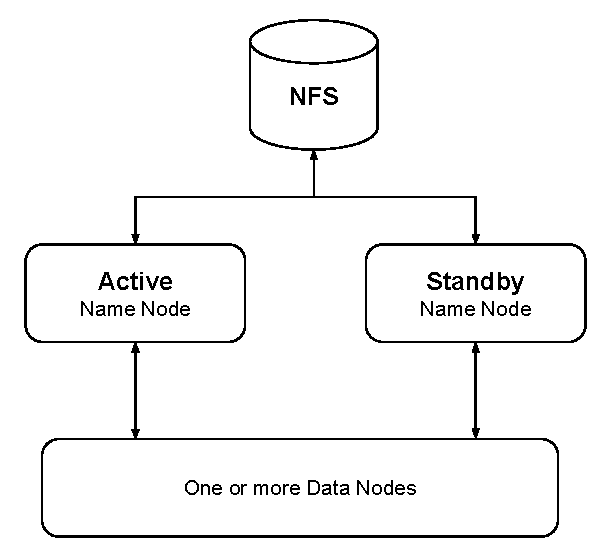
\includegraphics[scale=0.7]{pdf/hadoop-2x-nfs.pdf}
		\caption[Hadoop 2.x NFS solution]{Component diagram of the Hadoop 2.x NFS solution. \label{fig:hadoop-2x-nfs}}
	\end{figure}	

	This approach will undeniably mask the single point of failure (SPOF) error on the NameNode master by the cost and reliability to handle SPOF errors on the network file system abstraction, which in fact in most cases is a single server.
\end{enumerate}

\subsection*{Disco}
Mundkur \etal at Nokia Research Center publish in 2011 a paper on their implementation of the distributed computing platform Disco\cite{PageDisco}\cite{Mundkur:2011:DCP:2034654.2034670}. Disco is an easy customizable MapReduce (described in section \ref{sec:mapreduce}) framework with regards to environment and requirements, designed for clusters of commodity server machines. Disco is likewise based on the master/slave architecture and relies on a standard file system and thus, deprioritize persistent fault tolerance, achievable by a dedicated custom implementation. 

The single master pattern is as mentioned a single point of failure but is preferred due to consistency over availability (CAP theorem is outlined in \ref{def:cap}).
\vspace*{5mm}

\begin{definition}[CAP Theorem] \label{def:cap}
\textit{Eric Brewer presented in his keynote speech}\cite{Brewer2000} \textit{the CAP (Consistency, Availability, and Partition Tolerance) theorem that states, a distributed system (set of independent computers working together) only at any point in time can guarantee two of the three listed acronym properties, as illustrated in Figure \ref{fig:cap}.}

\begin{figure}[h!]
	\centering
	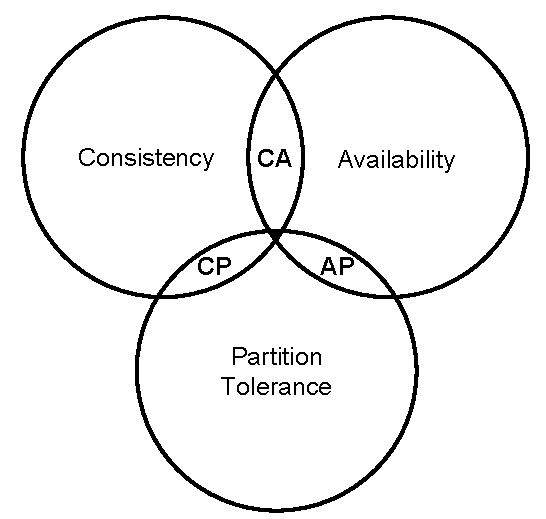
\includegraphics[scale=0.7]{pdf/cap.pdf}
	\caption{Illustrating the concept and limitations of CAP. \label{fig:cap}}
\end{figure}	
\end{definition}

\subsection*{Dynamo}
Dynamo is a highly available key-value storage system presented by Amazon engineers in \cite{DeCandia:2007:DAH:1294261.1294281}. The system is implemented using an eventual consistency protocol and thereby sacrifices it under certain scenarios, by cause of availability. 

The reason for this choice is the \textit{"always-on"} user experience on core services on the Amazon platform that Dynamo is used to function. Dynamo uses consistent hashing (outlined in definition \ref{def:ch}) to partition the key space across all available machines. A uniform distribution ultimately causes a uniform load assuming the key space access is not too skewed.
\vspace*{3mm}

\begin{definition}[Consitent hashing] \label{def:ch}
\textit{Engineer at Apache, White, describes in his blog post} \cite{PageWhiteCH} \textit{the purpose and demand for consistent hashing. It arose from the problems and limitations experienced with a naive hash-based key space distribution in a distributed system, where adding and removing machines in the network can be a catastrophe from a network bandwidth point of view, due to redistribution of the key space. In consistent hashing, only a fair share proportion from each of the machines is reassigned, while adding or removing machines.}
\end{definition}

\subsection*{Google File System}
Ghemawat \etal at Google describes the scalable distributed file system (GFS: Google File System) designed at implemented for primary developed for internal usage in \cite{Ghemawat:2003:GFS:945445.945450}. The file system is designed to run on inexpensive commodity hardware just as \eg Dynamo explained previously in this section, in addition to providing fault tolerance. 

The architecture is a single stateful master and slave(s) organization, where the (GFS) master maintains all metadata file in the system. 
\newline

A vastly simplified design and sophisticated placement of data on the slaves, together with a strong recovery protocol has been prioritized compared to the risk of a single master (as previously explained). Also are communication between clients and the master widely reduced, by caching slave metadata for further intercommunication on the client, such that the bottleneck effect on the master absents.
\vspace*{3mm}

\begin{definition}[Bottleneck effect] \label{def:bottle}
\textit{A part of a system is defined as a bottleneck if it critically limits the remaining system. This component usually has the lowest throughput of all.}
\end{definition}
\vspace*{3mm}

\section{Proposal} \label{sec:proposal}
The knowledge, features and compromises in the papers discussed and described in the latter section, \textit{Related work}, provides the foundation for the introductory piece of research in the project. It is first and foremost the ambition to investigate and evaluate different types of distributed file system architectures. The ambition of the research is to design and implement a prototype of an alternative to the existing file archives used in big data analysis subsequently, if achievable.
\newpage

The design of the architectural organization of the project is intended to eliminate the complications and issues in the existing solutions described among others. A desired outcome of latter is a substitute system eliminating data residuals and with reduced I/O-cost, complexity and increased performance.
\newline

The before mentioned specification and requirements can be empowered by splitting data semantically consistent at key positions by the file system, thus, data will be divided into arbitrarily sized chunks instead of fixed. Striking challenges includes:
\vspace*{5mm}
\begin{itemize}
	\item Describing a domain specific model to characterize the data semantics.
	\item Defining a direct data mapping for storing and retrieval.
	\item Designing a system that scales as the data and request rate grows, \ie provides consistent and intelligent load balancing.
\end{itemize}
\vspace*{5mm}

A feasible solution to reduce I/O-cost includes the mechanism of data cleaning, which is an important preprocessing step in big data analysis where \ie following actions can be performed:
\vspace*{5mm}
\begin{itemize}
	\item Reformat multidimensional scientific dataset such that identical features are grouped.
	\item Noise reduction.
	\item Transformation and dimensionality reduction (remove redundancy).
\end{itemize}
\vspace*{5mm}

The system seeks to perform the actions as mentioned above in real time since they are computationally simple on modern high-end processors and are attractive to perform before writing data to disk. 
\newline

Furthermore, a straightforward extension is to measure and store elemental statistics per dataset in a fashionable and state-of-the-art way. It is ultimately an ambition to integrate the same execution model as in \eg Hadoop and Disco, namely MapReduce around the implemented file archive to compose a full big data analysis framework alternative.

\section{Assumptions} \label{sec:assumption}
Following assumptions are constructed first and foremost to limit the prototype to the field of study interesting for this project and secondly because match the surrounding environment and settings.

\begin{itemize}
	\item The solution is targeted research and scientific related data. 
	\item The solution is targeted and used for BDA.
	\item Data entries can be processed and analyzed independently, which can be derived straight forward from the previous statement.
	\item A whole dataset is accessed, processed or modified at once.
	\item The majority of the datasets is passive, \eg not quite accessed as much as expected in systems like GFS.
\end{itemize}

\section{Expected results} \label{sec:expected-results}
The fundamental project description, protocol, and intention described in \eg section \ref{sec:problem} and \ref{sec:proposal} combined with the assumptions mentioned in the latter section can be delineated by following statements:

\begin{itemize}
	\item Investigate and evaluate different file system architectures, in order to optimize performance for big data.	
	\item Analyze one or more approaches, to efficiently pipeline described computations on incoming data.
	\item Define or use existing descriptive configuration language to specify computational filters.
	\item Understand and apply suitable high performance computing and other efficiency measures.
	\item Examine and reflect on performance benchmark results.
\end{itemize}

\section{\todo{Outline}}

